\documentclass[logo,reportComp]{thesis}
\usepackage[cpp,pseudo]{mypackage}

\title{操作系统原理实验报告}
\subtitle{实验三:开发独立内核的操作系统}
\school{数据科学与计算机学院}
\author{陈鸿峥}
\classname{17大数据与人工智能}
\stunum{17341015}
\headercontext{操作系统原理实验报告}
% \authorremark{本实验报告用\LaTeX撰写,创建时间:\builddate\today}


\begin{document}

\maketitle

\section{实验目的}
% 牵引车(实验一)->火车头(实验三)->车厢(实验二)
\begin{itemize}
    \item 掌握C语言与汇编混合编程的方法
    \item 分离引导程序和内核,学会用引导程序引导系统内核
    \item 为操作系统提供批处理能力
\end{itemize}

\section{实验要求}
% 实验目的和实验要求由老师提供实验项目文档中获取
\begin{itemize}
    \item 将实验二的原型操作系统分离为引导程序和MYOS内核,由引导程序加载内核,用C和汇编实现操作系统内核
    \item 扩展内核汇编代码,增加一些有用的输入输出函数,供C模块中调用
    \item 提供用户程序返回内核的一种解决方案
    \item 在内核的C模块中实现增加批处理能力
    \begin{itemize}
        \item 在磁盘上建立一个表,记录用户程序的存储安排
        \item 可以在控制台命令查到用户程序的信息,如程序名、字节数、在磁盘映像文件中的位置等
        \item 设计一种命令,命令中可加载多个用户程序,依次执行,并能在控制台发出命令
        \item 在引导系统前,将一组命令存放在磁盘映像中,系统可以解释执行
    \end{itemize}
\end{itemize}

\section{实验环境}
% 包括:硬件或虚拟机配置方法、软件工具与作用、方案的思想、相关原理、程序流程、算法和数据结构、程序关键模块,结合代码与程序中的位置位置进行解释。不得抄袭,否则按作弊处理。
% 实验方案包括相关基础原理、实验工具和环境、程序流程和算法思想、数据结构与程序模块功能说明,代码文档组成说明等
具体环境选择原因已在实验一报告中说明。
\begin{itemize}
	\item Windows 10系统 + Ubuntu 18.04(LTS)子系统
	\item gcc 7.3.0 + nasm 2.13.02 + GNU ld (Binutils) 2.3.0
    \item GNU Make 4.1
	\item Oracle VM VirtualBox 5.2.8
    \item Bochs 2.6.9
	\item Sublime Text 3
\end{itemize}

本次实验添加了Bochs虚拟机,用于单步调试。

虚拟机配置:内存4M,无硬盘,1.44M虚拟软盘引导。

\section{实验方案}
% 包括:主要工具安装使用过程及截图结果、程序过程中的操作步骤、测试数据、输入及输出说明、遇到的问题及解决情况、关键功能或操作的截图结果。不得抄袭,否则按作弊处理。
\subsection{C与汇编函数互调}
相比较之下,从汇编程序中调用C函数会比较简单,在程序段头部添加\verb'extern'标识符,然后在程序中直接\verb'call'即可。
由于核心内核功能都在C程序中完成,因此汇编调用C函数也只在内核引导部分用到(\verb'call main'),也不需要传递参数。

而从C程序中调用汇编函数则有两种方法。

一种是直接在C中写内联(inline)汇编,通过\verb'asm volatile'即可声明,某对双引号对中写一条语句,并用\verb'\n\t'换行(因为这一部分是原封不动地放入汇编语句的,所以需要换行以区分不同指令)。
之后的三个冒号,第一个冒号后填写输出变量,第二个冒号后填写输入变量,最后一个冒号后填写毁坏变量(防止编译器使用)。
同时注意在编译时要添加\verb'masm=intel',使得编译器更改默认AT\&T汇编语法为Intel的语法。

如设置光标(cursor)的函数,直接将参数传入\verb'ax',\verb'bx',\verb'dx'三个寄存器。
\begin{lstlisting}
void set_cursor(size_wd row, size_wd col){
    // AH = 0x02
    // BH = display page (usually, if not always 0)
    // DH = row
    // DL = column
    asm volatile(
                "int 0x10\n\t"
                :
                :"a"(0x0200), "b"(0), "d"((row << 8) | col)
                );
}
\end{lstlisting}

第二种方法则是通过直接函数调用的方式,在C语言中声明一外部函数\verb'extern fun',然后在汇编程序头部声明全局变量\verb'global fun',这样就可以直接在C程序中调用汇编函数了。
但是这种方法麻烦的一点在于传递参数,需要对函数调用、内存堆栈模式十分熟悉。
如一参数传递进来,则其应该在\verb'esp+8'的位置(\verb'esp+4'为函数返回地址)。
同时注意调用规范(convention),将必要的寄存器进栈(保护现场),设定好栈指针\verb'esp'和基址指针\verb'ebp',最后函数执行完后要将之前保存的寄存器出栈(恢复现场)。

\subsection{引导流程}
首先\verb'bootloader'在软盘的首扇区,作为主引导程序被加载入内存\verb'0x7c00'的位置,进行寄存器的初始化后,将操作系统内核加载入内存。

这里的操作系统内核即为汇编程序\verb'os.asm'和C程序\verb'kernel.asm'混合编译而成的内核二进制流\verb'kernel.bin'。
这里我们将内核加载到内存\verb'0x7e00'的位置,即主引导程序(512K)之后的位置。

内核的第一部分是汇编程序,设置软件中断及显示欢迎语;然后直接调用C程序中的\verb'main'函数,调出shell,即命令行部分,实现操作系统与用户的交互。

\subsection{Shell}
交互界面Shell是本次实验最大的亮点,具体实验结果请见下一部分。

我实现了以下几点功能:
\begin{itemize}
    \item 实现显存的基本输入输出功能
    \begin{itemize}
        \item 用户输入\textbf{实时}显示
        \item \textbf{光标}显示且跟随用户输入移动
        \item 自动\textbf{换行及清屏}
    \end{itemize}
    \item 字符串功能
    \begin{itemize}
        \item 常用C库函数\verb'strlen'、\verb'strcmp'、\verb'strcpy'、\verb'strncpy'、\verb'strcat'
        \item 字符串与整数的变换\verb'atoi'、\verb'itoa'
        \item 读取用户单个输入\verb'getchar'、整行输入\verb'getline'
    \end{itemize}
    \item 通过\verb'enum'和自己写的\verb'set_color'函数实现简单的字符属性变换,进而实现不同信息的不同样式显示。命令行提示用绿色显示,普通用户输入用黑底白字显示,错误信息\verb'Error'用红色高亮。
\end{itemize}

而预设的解释执行指令只有以下几条,之后会添加更多的功能。
\begin{itemize}
    \item \verb'help':帮助命令
    \item \verb'show':显示用户程序组织
    \item \verb'exec':\textbf{批量}加载并执行所有用户程序
    \item \verb'exec [num]':加载并执行特定用户程序
    \item \verb'exit':退出操作系统
\end{itemize}

为了增强鲁棒性,我还实现了一些容错功能。
如输入不存在的指令会报\verb'command not found',但输入回车不会报错等。

\subsection{用户程序}
沿用实验二的四个用户程序,添加了两个软中断:
\begin{itemize}
    \item \verb'int 20H':输入Ctrl+C,即可在程序运行中间由用户程序返回内核/Shell
    \item \verb'int 21H':用户程序自然执行完,自动返回内核/Shell
\end{itemize}

\subsection{程序组织}
主引导程序为\verb'bootloader.asm',核心内核为\verb'os.asm'和\verb'kernel.c'混合编译而成的二进制文件。
目前实现的头文件如下
\begin{itemize}
    \item \verb'type.h':基本数据类型
    \item \verb'string.h':基本字符串功能
    \item \verb'sysio.h':基本输入输出功能
    \item \verb'terminal.h':交互界面/命令行操作
    \item \verb'userprg.h':组织管理用户程序
\end{itemize}

一个用户程序信息用一个结构体\verb'Program'存储,如下
\begin{lstlisting}
typedef struct Program{
    char name[8];
    size_os space;
    char pos[8];
    char description[50];
} Program;
\end{lstlisting}

所有的用户程序则都存储在上述的结构体数组中,在C程序的常量段存储,需要时可以显示信息或执行。

\subsection{完整编译流程}
本次实验采用\verb'Makefile'进行自动编译,大大缩减命令行输入的时间。

主要步骤如下
\begin{itemize}
    \item 用\verb'nasm'编译主引导程序,生成二进制文件\verb'bootloader.bin'
    \item 用\verb'nasm'编译\verb'os.asm',生成目标文件\verb'os.o'
    \item 用\verb'gcc -m16'编译\verb'kernel.c',生成目标文件\verb'kernel.o'(同时生成汇编文件\verb'.s'方便调试)
    \item 用\verb'ld'结合链接文件\verb'link.ld',将上述两个\verb'.o'文件链接生成内核二进制文件\verb'kernel.bin'
    \item 用\verb'nasm'编译其余用户程序,生成\verb'.com'文件
    \item 用\verb'mkfs.msdos'创建新的格式化1.44M虚拟软盘
    \item 用\verb'dd'指令将主引导程序放在第一个扇区,操作系统内核放在第二个扇区以后,用户程序放在第一面往后(第17逻辑扇区)
\end{itemize}

编译流程中最难的部分即怎么将汇编程序和C程序链接到一起。
由于生成的是目标文件,原来汇编指令中的\verb'org'就不能使用了,这时就应该采用链接指令,显式声明这段代码应该怎么安排,会被加载到内存的什么位置(\verb'0x7e00')。
这里我查阅了很多资料,自己学会了写链接脚本(linker script),即附件中的\verb'link.ld'。

\subsection{调试}
由于本次实验大部分时间都用在调试上,所以在此还是提及一下。

以前一直只知道gdb可以进行单步调试,但是对于16位32位的C程序,我还未掌握gdb的使用方法。
倒是在本次实验中发现bochs这个软件十分好用,在配置文件\verb'bochsrc.bxrc'中设置好后(主要是设置虚拟软盘的位置),就可以进行单步调试,同时还可以同步显示汇编指令,非常方便。

\section{实验结果}
实验二的原型程序被分离为引导程序(\verb'bootloader.asm')和操作系统内核(\verb'os.asm'和\verb'kernel.asm'),详情可见附件。

操作系统内核通过引导程序加载成功会显示欢迎字样,见图\ref{fig:bootloader}。
\begin{figure}[H]
\centering
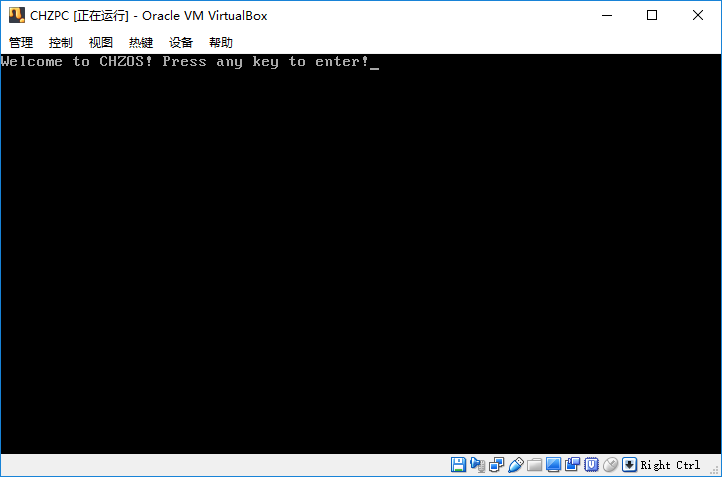
\includegraphics[width=0.8\linewidth]{fig/bootloader.PNG}
\caption{引导程序加载完毕}
\label{fig:bootloader}
\end{figure}

按任意键后可进入操作系统内核(Shell),即交互界面。
图\ref{fig:shell}中可以看到,输入\verb'help'会弹出所有支持的指令,
同时,用户输入和系统显示采用不同颜色高亮,而且配有光标。
当输入错误指令时,系统会提示\verb'command not found';输入空行则直接换行。
\begin{figure}[H]
\centering
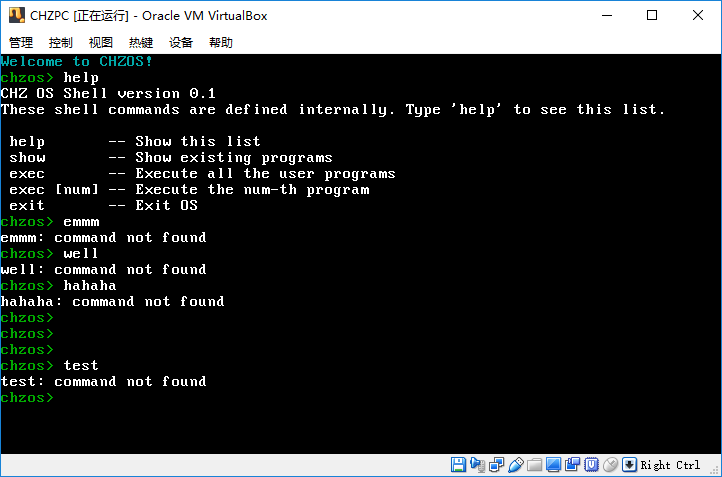
\includegraphics[width=0.8\linewidth]{fig/shell.PNG}
\caption{Shell用户界面}
\label{fig:shell}
\end{figure}

用\verb'show'指令可以查看之前在软盘中建立的表(图\ref{fig:organization}),即用户程序的名称、大小、存储位置(由于还未做文件系统,故这里统一标识为根目录)、描述。
\begin{figure}[H]
\centering
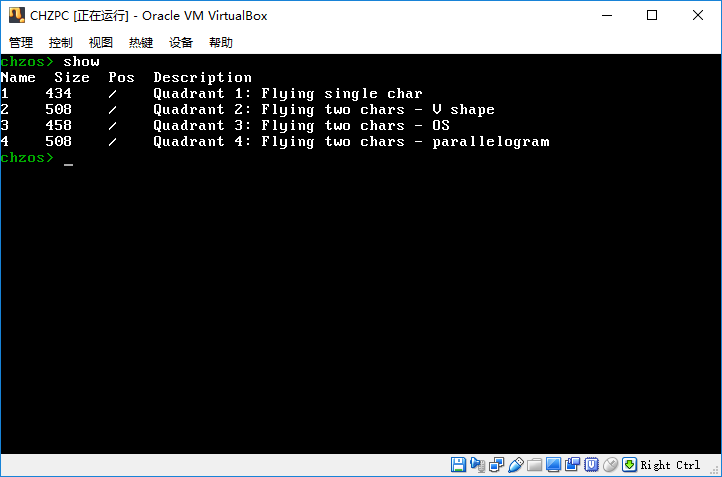
\includegraphics[width=0.8\linewidth]{fig/organization.PNG}
\caption{显示用户程序安排}
\label{fig:organization}
\end{figure}

如图\ref{fig:exec}所示,输入执行指令\verb'exec [num]'可执行对应用户程序。
4个用户程序的执行结果见图\ref{fig:execution}。
\begin{figure}[H]
\centering
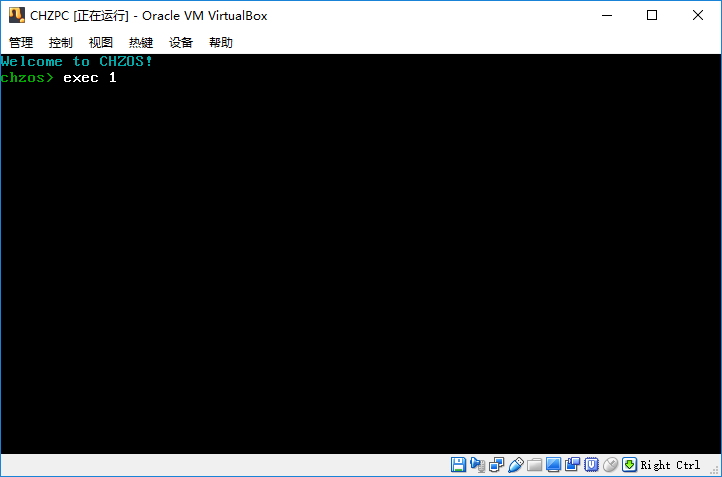
\includegraphics[width=0.8\linewidth]{fig/exec.PNG}
\caption{输入执行命令}
\label{fig:exec}
\end{figure}

\begin{figure}[H]
\centering
\begin{tabular}{cc}
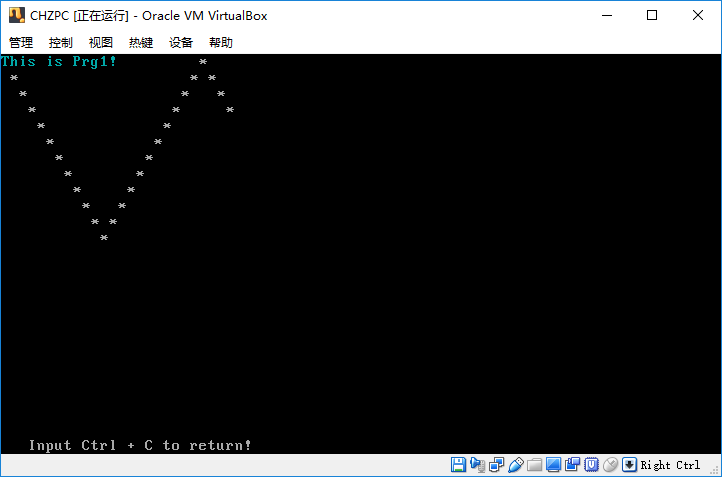
\includegraphics[width=0.5\linewidth]{fig/prg1.PNG}&
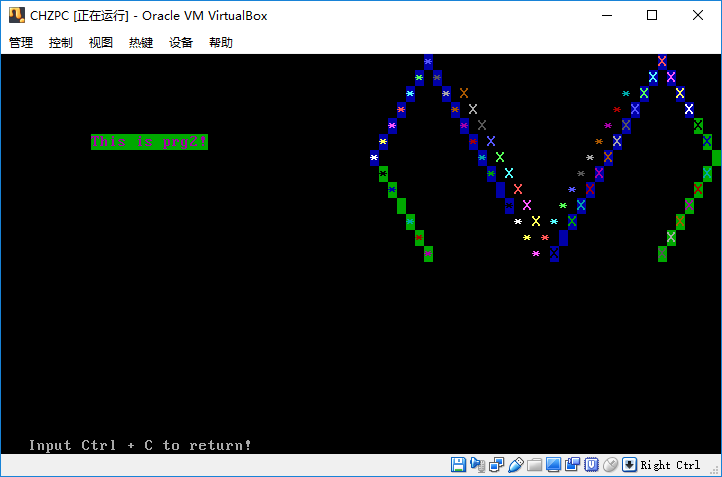
\includegraphics[width=0.5\linewidth]{fig/prg2.PNG}\\
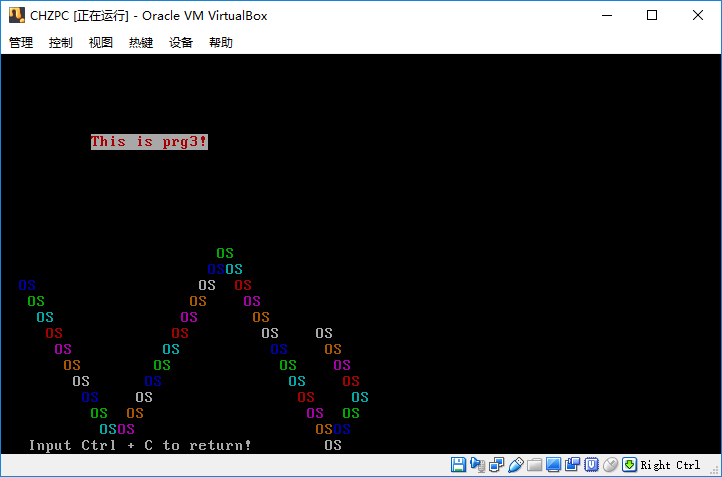
\includegraphics[width=0.5\linewidth]{fig/prg3.PNG}&
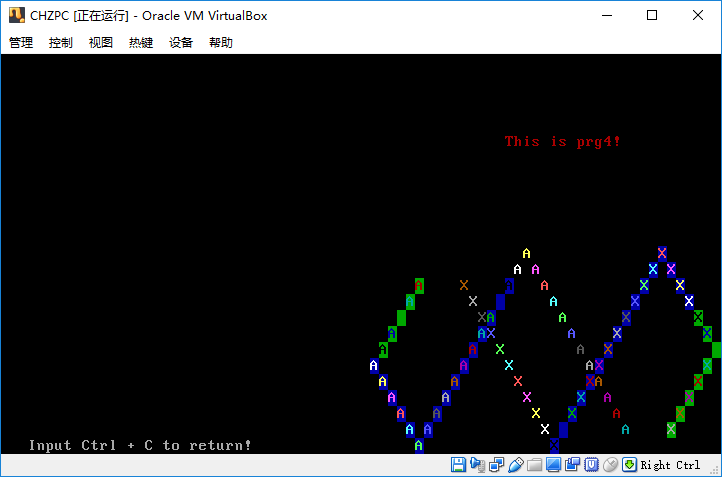
\includegraphics[width=0.5\linewidth]{fig/prg4.PNG}\\
\end{tabular}
\caption{用户程序执行}
\label{fig:execution}
\end{figure}

注意这几个用户程序可以通过\verb'exec'而不加标号声明,进行\textbf{批处理执行}。
但由于实验报告无法显示动态过程,故在此没有附截图,具体结果请加载软盘\verb'mydisk.img'执行。

\begin{figure}[H]
\centering
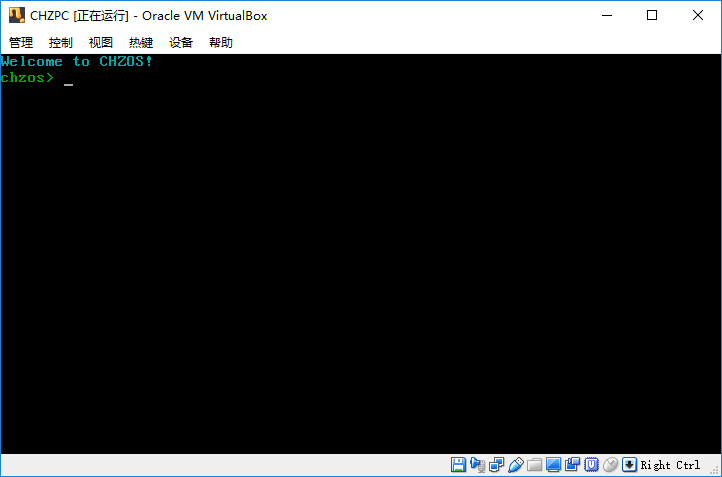
\includegraphics[width=0.8\linewidth]{fig/return.PNG}
\caption{用户程序返回内核}
\label{fig:return}
\end{figure}

上文提到返回内核的两种方法,Ctrl+C中断返回或程序执行完毕自动返回。
类似实验二的操作,只不过实验二是返回监控程序,实验三中是返回shell(图\ref{fig:return})。

最后,输入\verb'exit'指令可退出操作系统,如图\ref{fig:exit}。
\begin{figure}[H]
\centering
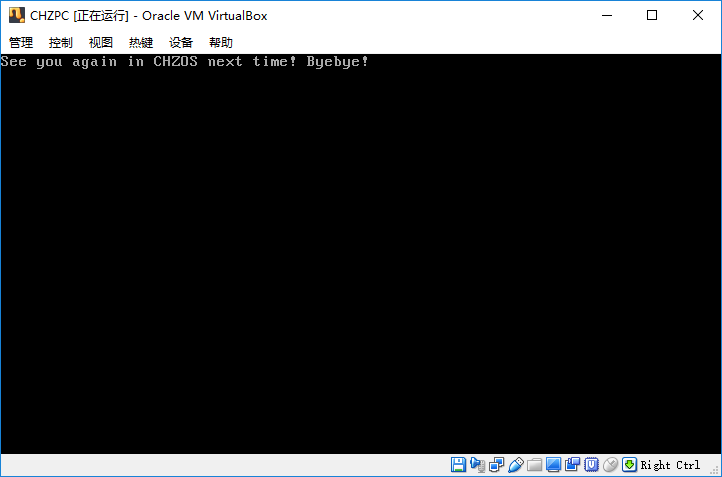
\includegraphics[width=0.8\linewidth]{fig/exit.PNG}
\caption{退出操作系统}
\label{fig:exit}
\end{figure}

\section{实验总结}
% 每人必需写一段,文字不少于500字,可以写心得体会、问题讨论与思考、新的设想、感言总结或提出建议等等。不得抄袭,否则按作弊处理。

本次实验花费了我整整两周时间,每天无时无刻不在想操统实验怎么完成,每天都肝到一两点才去睡觉,可以说操统实验令我心力憔悴。
而导致花了这么长的根本原因是环境的配置。

首先花了几天时间查阅资料,看究竟如何有办法实现汇编和C函数的互相调用。
一开始想着尽可能多用C语言编程,遇到实在没有办法实现功能的时候才使用汇编(如中断表写入、中断调用等),于是拼命查找C语言内联汇编的操作。
花了九牛二虎之力终于明白输入部、输出部、毁坏部的含义,以及如何在C语言中使用Intel的内联汇编。
这里纯属没事找事干,因为C语言默认的内联汇编是AT\&T语法,为了避免新学一门汇编,并且使得同一项目的不同汇编格式不同,所以坚决要采用Intel语法,于是终于找到要在C内联汇编的头部加上\verb'.intel_syntax noprefix'(实操时发现并不需要),并在编译时添加\verb'-masm=intel'选项。

基本的汇编内核和C语言内核都写出来了,本以为就可以开开心心编译完就完成项目了,谁知道后面的事情却更加麻烦。
秉承着gcc是世界上最好的C/C++编译器的观点,我死活都不肯``委曲求全''更换其他编译器。
由于实模式下操作系统必须是16位的,因而编译出来的程序也最好是16位的,否则寻址会出现一些问题。
其实现代的gcc编译器都可以生成16位代码,即添加\verb'-m16'编译指令。
想着我的gcc版本号这么高,应该编译不会有什么问题,于是便愉快地添加\verb'-m16',等着一遍编译通过。
然而事实是,我遇到了非常多的问题:
\begin{itemize}
	\item 由于不熟悉gcc的编译指令,大多时候都是上网搜索看别人怎么做的,我便直接复制粘贴他们的指令。
	但是换成自己的电脑自己的程序,往往又会出现新的编译报错。
	比如一开始我以为只要添加\verb'-march=i386'即可,但这边提示\\\verb'error: CPU you selected does not support x86-64 instruction set',\\那我就添加\verb'-m16'。
	然后又报\\\verb'cannot find -lgcc',\\我就要下载安装\verb'gcc-7-multilib'。
	又比如提示\\\verb;undefined reference to `_GLOBAL_OFFSET_TABLE_';,\\又添加\verb'-fno-pie'指令。
	每出现一个错,我就要去搜索一下,添加新的编译指令,然而我并不清楚这些编译指令的内在作用,或者它们之间是否会互相影响,完全就是在捉瞎。
	\item gcc的编译没有问题了,链接又不知道应该怎么写。
	因为没有了\verb'org'指令,所以重定位的操作就交由链接器来做了。
	而且要将汇编和C程序产生的目标文件合并起来,这使得难度进一步加大。
	一开始由主引导程序总是没有办法加载入系统内核,我一度怀疑老师所给的\verb'-Ttext'指令太过简单或有问题,于是自己跑去学习链接脚本(linker script)。
	用我自己的脚本写出来链接通过后,却还是一样的情况,要么系统内核无法进入,要么C的主函数无法进入。
	我很清楚是我的函数地址给错了,但是我又不知道怎么修改,就十分绝望。
	\item 而且这种问题还十分难以定位错误,中间某一个小细节出错了,就会导致后面全部出错。
	最开始在显存中显示字符全部由C语言编写,就直接设置\verb'uint16_t'类型指针指向显存开始地址\verb'0xB8000',然而程序总会陷入死循环无法正常在显存显示。
	不知道为什么就会跳到奇怪的地址,然后不断循环下面的代码段。
\begin{lstlisting}[language=bash]
(0) [0x0000000fe9e6] f000:e9e6 (unk. ctxt): push ax                   ; 50
<bochs:26> s
Next at t=439640331
(0) [0x0000000fe9e7] f000:e9e7 (unk. ctxt): call .-22398 (0x000f926c) ; e882a8
<bochs:27> s
Next at t=439640332
(0) [0x0000000f926c] f000:926c (unk. ctxt): mov al, 0x20              ; b020
<bochs:28> s
Next at t=439640333
(0) [0x0000000f926e] f000:926e (unk. ctxt): out 0x20, al              ; e620
<bochs:29> s
Next at t=439640334
(0) [0x0000000f9270] f000:9270 (unk. ctxt): ret                       ; c3
<bochs:30> s
Next at t=439640335
(0) [0x0000000fe9ea] f000:e9ea (unk. ctxt): pop ax                    ; 58
<bochs:31> s
Next at t=439640336
(0) [0x0000000fe9eb] f000:e9eb (unk. ctxt): iret                      ; cf
\end{lstlisting}
	后来迫不得已采用C语言内联汇编的方法才得以解决。
	其他问题也是在不断的尝试中,慢慢调整,不知道怎么就突然成功了,至今未明原因。
\end{itemize}

终于终于,C与汇编混合编译而成的操作系统可以被正常加载了,想着前面配置环境的坎终于被我迈过了,后面就仅剩实现功能了,果然我还是太过天真。
实现过程中又出现了很多诡异的问题,这些在以前编写高级语言程序时从来都没有遇到过。
也是类似上面的问题,程序运行到某个位置就开始陷入死循环,然后无法继续往下执行。
用Bochs单步调试多次,与C语言生成的汇编文件\verb'.s'互相比对,终于找出问题所在。
下面一段普普通通的C转为汇编的代码
\begin{lstlisting}[language=bash]
push	ebp
.cfi_def_cfa_offset 8
.cfi_offset 5, -8
mov	ebp, esp
.cfi_def_cfa_register 5
push	OFFSET FLAT:.LC6
call	show_string
\end{lstlisting}
实际运行时却变成了下面这样
\begin{lstlisting}[language=bash]
(0) [0x000000008551] 0000:8551 (unk. ctxt): push 0xe8668618           ; 6668188666e8
<bochs:9> s
Next at t=478219853
(0) [0x000000008557] 0000:8557 (unk. ctxt): salc                      ; d6
<bochs:10> s
Next at t=478219854
(0) [0x000000008558] 0000:8558 (unk. ctxt): (invalid)                 ; feff
<bochs:11> s
Next at t=478219855
(0) [0x0000000fff53] f000:ff53 (unk. ctxt): iret                      ; cf
<bochs:12> s
\end{lstlisting}
诡异,十分诡异!
而这个问题源于我在C程序中直接在函数参数中传递了字符串常量,如\verb'show_string("Hello")'\\
这样。
但修改为先赋值给变量,再传递变量的方式就没有问题,即
\begin{lstlisting}
char* HELLO = "Hello";
show_string(HELLO);
\end{lstlisting}
这只能说gcc编译出来的16位代码实在是太有问题了,于是我只能负重前行,将所有传常量字符串的地方全部修改为赋值再传递,相当麻烦。(我也考虑过采用其他C语言的交叉编译器,如Watcom C、i386-elf-gcc等,但都没有成功实现)

基本的Shell写完了,最后一步是加载用户程序。
本来沿用实验二的代码段即可,但是这里涉及到C语言中调用汇编函数,相比起汇编调用C直接写\verb'call'就好了会麻烦很多。
查阅资料知道函数调用参数存放在栈中的第二个位置,即\verb'esp+8'的地方。
于是从该位置读出参数,却始终没法正常加载用户程序,老是跳转到其他位置陷入无尽的黑暗。
一直以为是我的函数调用出了问题,但找了很久原因才发现是我的软盘组织出了问题。
一开始我为了方便系统内核加载,由于不知道会占用多少空间,于是便设定了主引导程序加载20个扇区,用户程序从第21个扇区开始存放。
而正是问题所在,我习惯性地以为第21个逻辑扇区是磁盘的0面0道22号扇区,而实际上,逻辑21扇区已经是1面/磁头了。
于是重新查阅了磁盘的组织,将用户程序放在1面0道1扇区开始(即逻辑17扇区),然后修改中断调用,这样子就可以成功调用用户程序了。

总的来说,本次操作系统实验学到的东西太多了,深刻明白C程序与汇编程序的互相调用、混合编译,清楚应该怎么组织系统内核程序。
自己实现了一些底层的C库,明白这些输入输出函数的工作原理,而不像以前写高级语言程序一样只将其当作黑箱调用。

而最深的感受则是\textbf{做系统}实在是件技术活,尤其是做底层的系统。
开发高层应用只会有不会怎么写的问题,如果想清楚算法,想清楚程序的组织,那一般这个软件实现起来就没有问题。
但是做系统就不一样,哪怕你想清楚怎么写,想清楚每一步需要做什么,最后将这些组件组合起来依然是一门学问。
也许并不是你写得不好,而是胶水不够给力,这样你的系统依然是不work的。
考虑各组件之间的\textbf{耦合性},这是实现系统的一个很关键的因素。

至于\textbf{做底层}的东西也是一件技术活,不像高层语言那样有IDE、调试器,有各种各样完整的工具链供你使用,越是底层能使用的东西就越少。
你要十分清楚你每一步都在干些什么,没有基础设施,全部都要自己写。
就是一个空白的显存给你,实现命令行这看似简单的操作,实则蕴含了非常多的学问。
颜色的控制?换行呢?清屏呢?退格键支持?字符串匹配?光标显示?等等等等,太多要考虑的地方了。
难以调试、难以定位错误、难以找资料等,都使得底层系统的实现难上加难。
这让我想起上个学期做CPU的实验,同样也是这样。
用Verilog写的程序,通过完全是黑箱的后端编译,然后上到FPGA板上运行。
本来软件模拟好好的没有什么问题,但一上到硬件就出现各种莫名其妙的错误。
FPGA没有自己的显示器,也不支持单步调试,当时也是花了九牛二虎之力才发现问题所在。

本学期的操作系统则是结合了底层的难度和做系统的难度,可以说是极其复杂了,它还不比CPU,它真真确确是一个完整的系统,起到承上启下的作用。

一句话总结吧,虽然写操作系统耗费的精力巨大,但是这真是一门有趣的课,最终获得的成就感也是无可比拟的。


\section{参考资料}
\begin{enumerate}
	\item 李忠,王晓波,余洁,《x86汇编语言-从实模式到保护模式》,电子工业出版社,2013
	\item GCC-Inline-Assembly-HOWTO, \url{https://www.ibiblio.org/gferg/ldp/GCC-Inline-Assembly-HOWTO.html}
	\item Can I use Intel syntax of x86 assembly with GCC?, \url{https://stackoverflow.com/questions/9347909/can-i-use-intel-syntax-of-x86-assembly-with-gcc}
	\item How can i write inline assembler in c code, \url{https://forum.nasm.us/index.php?topic=2114.0}
	\item Linking C with NASM, \url{https://stackoverflow.com/questions/24991944/linking-c-with-nasm}
	\item Compile an asm bootloader with external c code, \url{https://stackoverflow.com/questions/47249699/compile-an-asm-bootloader-with-external-c-code}
    \item Bare Bones, \url{https://wiki.osdev.org/Bare_Bones}
    \item Stack frame layout on x86-64, \url{https://eli.thegreenplace.net/2011/09/06/stack-frame-layout-on-x86-64/}
    \item 10分钟读懂Linker scripts, \url{https://blog.louie.lu/2016/11/06/10%E5%88%86%E9%90%98%E8%AE%80%E6%87%82-linker-scripts/}
    \item 
    \item Debugging and Building Operating Systems, \url{https://www.codeproject.com/Articles/16582/Debugging-and-Building-Operating-Systems}
\end{enumerate}

\appendix
\appendixconfig
\section{程序清单}
\label{sec:code}
由于程序太多,请直接见压缩文件。

\section{附件文件说明}
\begin{center}
\begin{tabular}{|c|l|l|}\hline
序号 & 文件 & 描述 \\\hline
1 & \verb'bootloader.asm' & 主引导程序\\\hline
2 & \verb'os.asm' & 内核汇编部分\\\hline
3 & \verb'kernel.c' & 内核C部分\\\hline
4 & \verb'Makefile' & 编译指令文件\\\hline
5 & \verb'link.ld' & 链接文件\\\hline
6 & \verb'bochsrc.bxrc' & bochs调试文件\\\hline
7 & \verb'mydisk.img' & 核心虚拟软盘\\\hline
8$\thicksim$11 & \verb'prgX.asm' & 用户程序\\\hline
12$\thicksim$16 & \verb'/include' & C头文件\\\hline
\end{tabular}
\end{center}

\end{document}

% 实验提交内容
% 实验报告:电子版(Word2003的DOC格式或PDF格式)
% 原程序文件及可执行代码程序文件
% 测试输入数据文件和输出数据文件
% 虚拟机软盘映像文件

% 基础实验项目5个和扩展实验7个
% 实验项目,迟交影响成绩评价!
% 工具与环境可由选择,开发新型工具或优化一套开发环境都可加分!
% 一系列基础实验项目必须连续完成,当前项目只能在前一个项目的基础上进行,体现出前后的进化关系,否则要被约谈,证明没有抄袭行为!
% 一个项目可提交多个改进的版本,实现新功能和个性化特征都有利于提高相应项目的成绩。
% 实验项目提交内容用winrar工具整体压缩打包,统一格式命名为:
%    <学号>+<姓名>+<实验项目号>+<版本号>.rar
%    姓名(学号)实验NvX.zip
%    实验报告、项目文件夹、映像文件
%    ftp://172.18.216.232 sysuac 下周六23:59

% 免考
% 条件:实验1~6全部评价AAAAB+B+或相当
% 最终成绩可能范围:75分以上